\section{Methodology}

We use a sequence of optimization processes based on observation and synthetic data to find the most appropriate \qsvs{} relationship parameters. The proposed process makes it possible to locate the most accurate shear wave velocity range or effective shear wave velocity range to study \qsvs{} relationship for each seismic station. We use the term of effective shear wave velocity range for the range of \vs{} that a traveling wave has been highly influenced from while propagating in the domain, or based on recorded data and optimization process we can extract $Q$ values for that range of \vs{}. The \qsvs{} relationship is defined as a function of shear wave velocity.  A genetic algorithm (GA) is used to search for the best parameters of this relationship.  In simple words, it efficiently searches for those parameters that result in close to target values. Target values can be acquired from synthetic ground motion simulations or actual observations. GA uses a function, which is known as a cost function, to evaluate the proposed parameters. If it provides good results, it keeps them if not it searches for other parameters unless it finds the best solution or meets the termination criteria. The cost function evaluation is based on signals comparison. It is not possible to compare two signals wiggle by wiggle at higher frequencies (\fmaxeq{0.5}). Therefore, the cost function compares some metrics of signals instead of the whole waveforms.  The synthetic signal is generated based on proposed parameters by GA at iteration. Extracting these metrics, for each set of new parameters, requires running a regional scale ground motion simulation. These runs are computationally expensive and time-consuming. To make this process practical under a reasonable time and computational budget, based on many simulation data, we develop surrogates (or meta-models).  The surrogates are artificial neural networks (ANNs) that are trained to accurately estimate the signal metrics based on \qsvs{} relationship input parameters. Fig.~\ref{fig:Figure_1} shows the method's workflow. The workflow includes four main tasks:
\begin{itemize}
        \item \qsvs{} relationships and ground motion simulations 
	\item Preprocessing signals and extracting signals metrics,
	\item Developing surrogates, 
	\item Running the optimization process to search for the best input parameters, and
	\item Locating the effective shear-wave velocity range and choosing data.  
\end{itemize}

 \begin{figure}[ht]
    \centering
    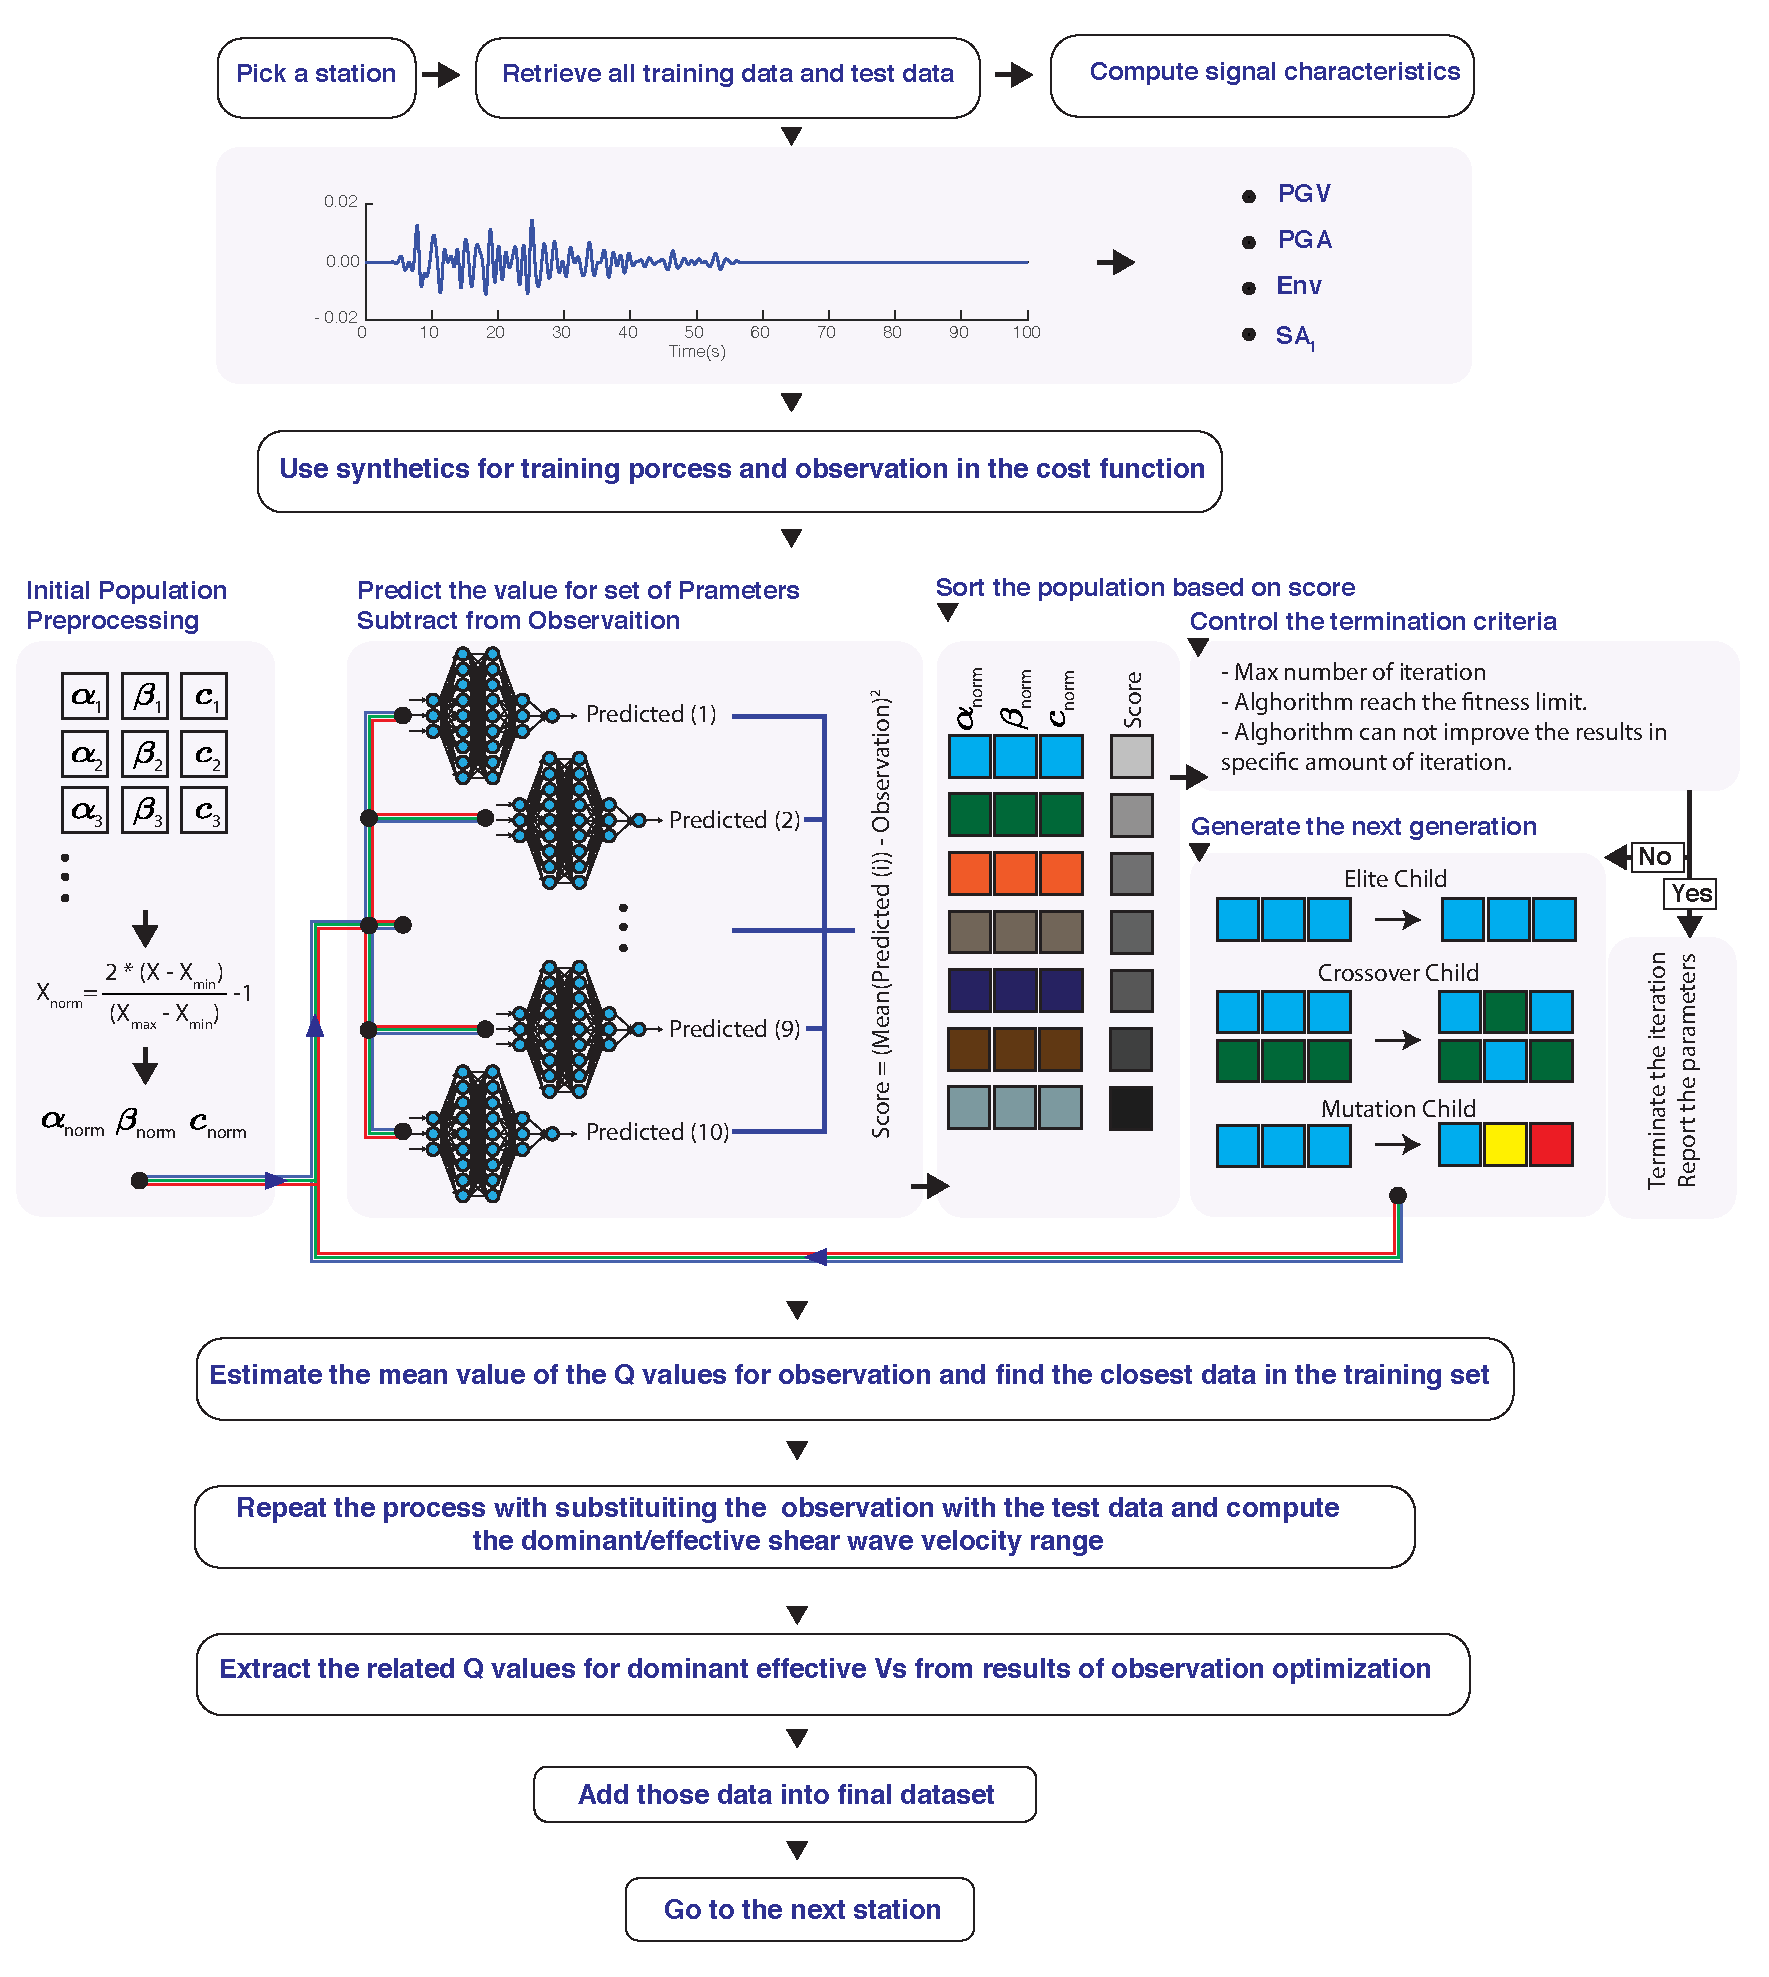
\includegraphics[width=\textwidth]{figures/pdf/Figure_02.pdf}
    \caption{Processing steps {\color{red} working on improving this figure and the caption.}}
    \label{fig:Figure_1}
\end{figure}

In the rest of this section, we go into details of each mentioned tasks.

\subsection{Attenuation models and ground motion simulations}
We use a finite element code to conduct physics based ground motion simulation \citep[for more details see ][]{Tu_2006_Proc,Taborda_2010_Tech}. 
In the code, energy loss due to anelasticity is represented by springs and dashpots. In this study, we use a model which combines two Maxwell elements and one Voigt element \citep{Bielak_2011_G}. The model converts the provided $Q$ value to desirable attenuation in the forward simulation. For the $Q$ equation we use the following equation: 

\begin{equation}
Q_{S}(V_{S}) = C + \alpha(V_{S})^{\beta}
\end{equation}

$C$ serves as floor value for low-velocity structures and $\alpha$ and $\beta$ offer different growth rates for increasing values of \vs{}. \qp{} depends on \qs{} and \qk{}, which is dilatational reciprocal quality factor. Since in soil and rock materials the intrinsic attenuation due to shear is generally much greater than that due to dilatation, we ignore dilatational reciprocal quality factor (\qk{}=~$\inf$). \qp{} is computed using

\begin{equation}
Q_{P}=2Q_{S}.
\end{equation}

Based on random combination of \qsvs{} relationship input parameters (i.e., $C$, $\alpha$, $\beta$) we run many physics-based ground motion simulation and generate the training dataset. 

\subsection{Signal Metrics}

There are numerous methods for quantitatively comparing two signals in time and frequency domain (see khoshnevis and Taborda 2018 and references therein). Q factor parameter studies commonly use peak ground velocity or peak amplitude of S wave arrivals as an indicator to energy loss during the wave propagation. Unless in completely homogenous domain, it is not easy to pick the peak ground velocity for S-wave arrival. In complex geological structure surface wave and  direct S wave and reflected body waves from different layers are mixed together. In that case the energy is already dissipated in propagation process and the peak ground velocity is not very sensible to the Q parameters. We will have more discussion on this issue in the result section. Also picking the actual peak value of S Wave arrivals is extremely prone to error and it is not straight forward to distinguish body wave and surface wave windows in a complicated geological regions \citep[e.g., see][]{bowden2017earthquake}. Moreover, our ideal case experiments prove that using only peak ground velocity will not necessarily provide better results even if we be able to accurately pick the peak ground velocity for S wave. Khoshnevis and Tabarda 2018 showed that response spectra is the most important parameter in qualitative comparison of signals as well as total energy. Following their recommendation, in this paper, we add 3 other parameters to the qualitative comparison of signals process. Keeping peak ground velocity, we also use response spectra for the highest frequency of the simulation ($T= 1s$), peak ground acceleration and area under the envelope of the signal which is another indication of total energy. For more details about the GOF metrics please refer to  khoshenvis and Taborda 2018 or Anderson 2004. We computed the signal envelop using the Hilbert transform. Figure.~\ref{fig:signal_envelop} Shows example of signal envelop and the area under it. 

  \begin{figure}[ht]
    \centering
    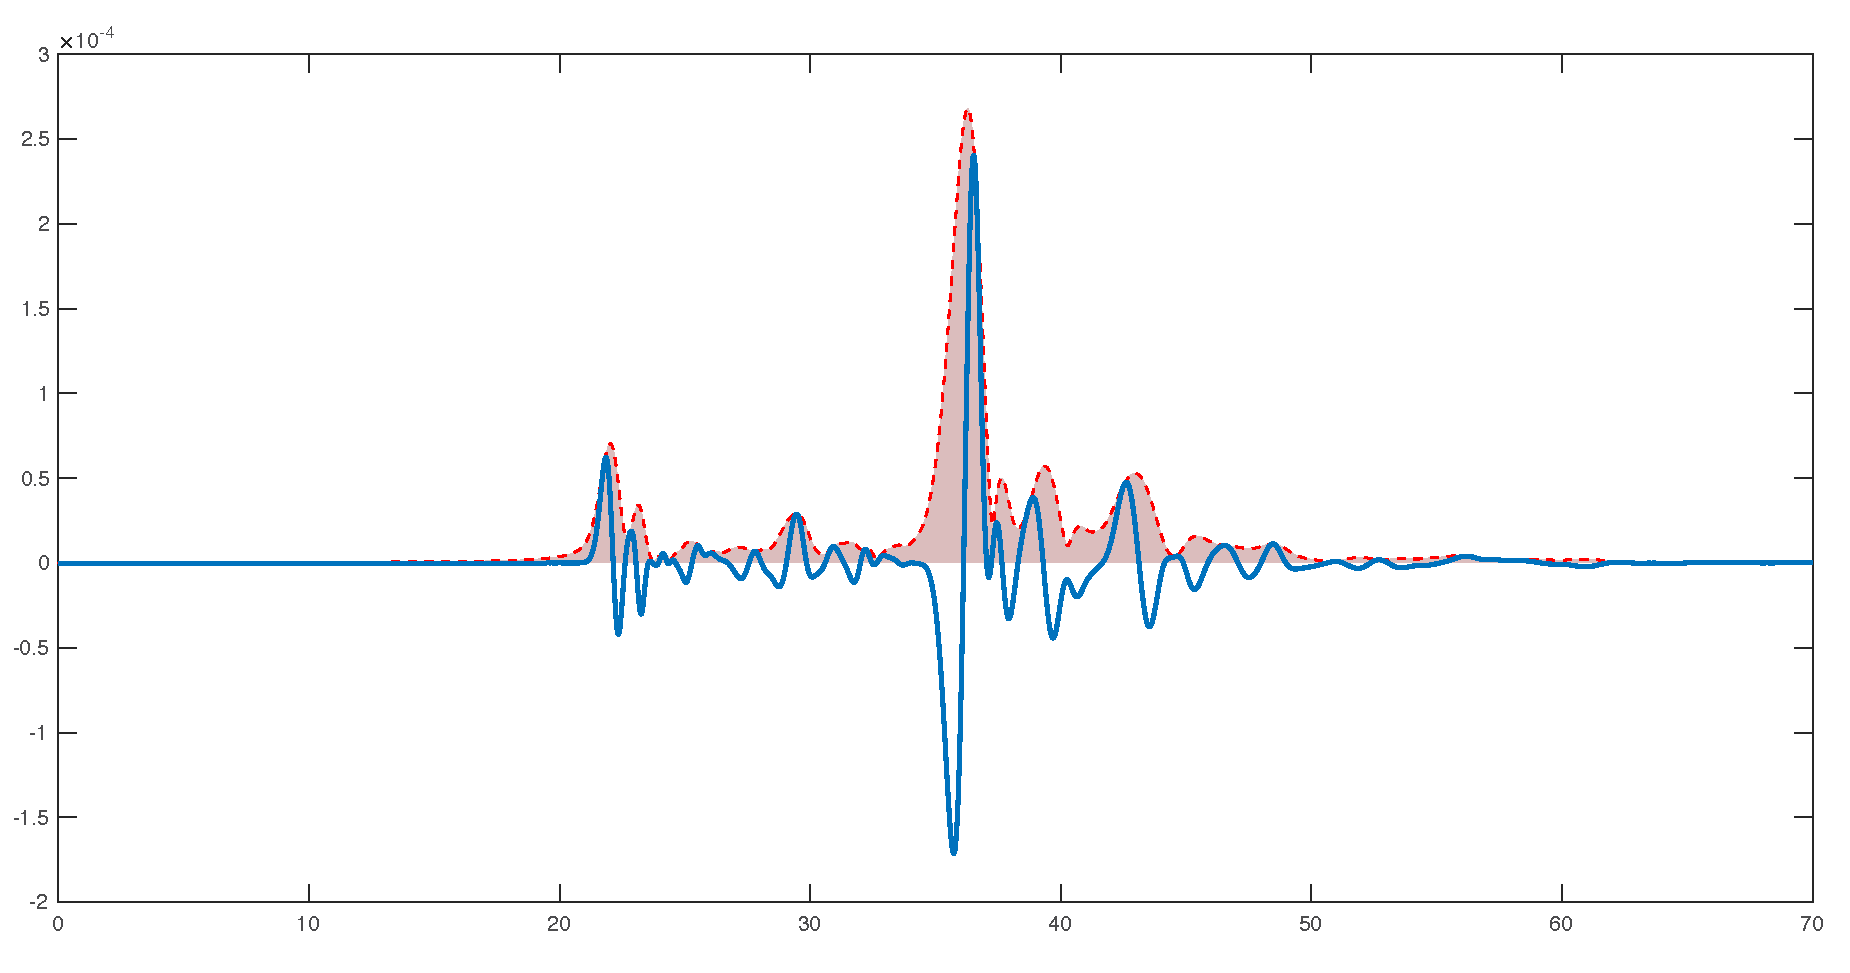
\includegraphics[width=\textwidth]{figures/pdf/signal_envelop.pdf}
    \caption{Example of signal envelop}
    \label{fig:signal_envelop}
\end{figure}




\subsection{Developing surrogates} 

Surrogates are developed using artificial neural networks (ANNs). ANNs are inspired in the human brain. A given network is a combination of different so-called neurons which have certain initial weight and activation functions. These neurons are grouped in different layers. The first layer is called input layer, and the last layer is called the output layer. Other layers between input and output layers are called hidden layers. We use two structures of ANNs.  One structure is developed to estimate PGV, and the other structure is developed to estimate PGV, PGA, SA, and Venv for two horizontal components. Alternative metrics increase signal uniqueness. There is less chance that two signals which are generated with two sets of different input parameters (i.e., $C$,$\alpha$, and $\beta$) have the same PGV, PGA, Venv and SA. Consequently, the optimization algorithm can effectively find the best set of solutions. Fig.~\ref{fig:Figure_ann_structure} shows the structures of networks. The number of neurons in each hidden layer is presented at the top of each layer.

 \begin{figure}
    \centering
    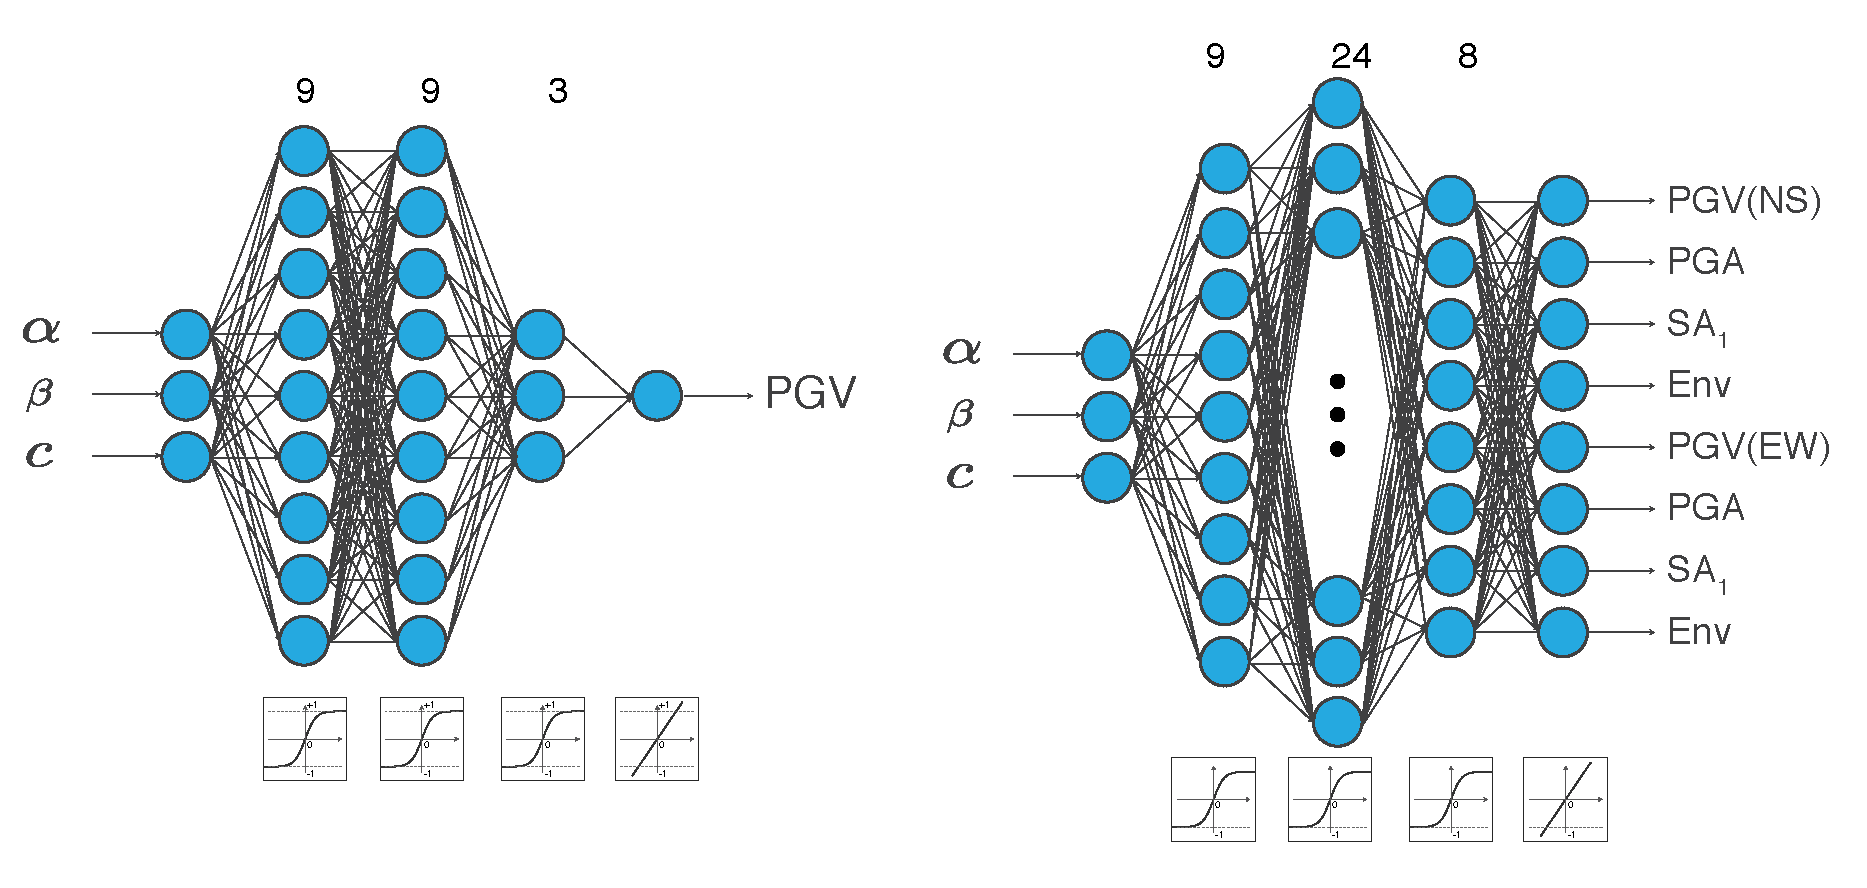
\includegraphics[width=1\textwidth]{figures/pdf/Figure_03.pdf}
    \caption{Feedforward multilayer perceptron neural networks used in the study. Hidden layers use tangent sigmoid and output layer uses linear activation functions. Dots used to simplify the structure for presenting purposes.}
    \label{fig:Figure_ann_structure}
\end{figure}

Input values for all ANNs in this study is \qsvs{} relationship parameters (i.e., $C$, $\alpha$, and $\beta$). All nodes are interconnected, and each layer has an activation function. One can train a network using available data by means of a process during which the weights and bias values associated with the network's neurons are updated so that these will produce output results with increasingly lower residuals in comparison with the input observations. Training ANNs provides a mean to avoid repeated expensive computations. Studying neural network structure and different networks and algorithms are beyond the scope of this study.  In this study, we use feedforward neural networks and Levenberg-Marquardt optimization as a network training function to update weight and bias values. We use linear transfer functions for the last layers and hyperbolic tangent-sigmoid transfer functions for the rest of them. The package is implemented in Matlab programming tool. The algorithm divides the data into three sets including training, validation, and testing dataset. Validation dataset is used to stop training process to avoid overfitting during the training process. An ANN can accurately learn any dataset, provided there is no noise in the data. However, a well trained ANN for one dataset may not be a good predictor for another dataset. This situation is called overfitting. Validation dataset is used to stop the training processing when overfitting occurs. The test dataset is used after fully training data to analyze the functionality of the network. For training ANNs, first, we leave out 5\% of the dataset for the final testing. These data have never been provided to ANNs during the training sessions. We assign 85 and 15\% of remaining data into training and validation datasets.  Neural networks' training process, depending on the size of the networks, is involved with hundreds of thousands of matrix multiplication. Therefore, normalized input values ensure the stability of the networks and improve its internal optimization process in case of inequivalent attributes. We linearly scale the data into $[-1,1]$ using

\begin{equation}
X_{norm} = \frac{2*(X-X_{min})}{(X_{max}-X_{min})}-1
\end{equation}

where $X_{norm}$ is the normalized value; $X_{min}$ and $X_{max}$ are minimum and maximum value of $X$ vector, respectively. The performance is computed by use of mean squared error (RMSE) between the network predicted values and observation. As of epoch number increases, the network learns to predict the data with high accuracy. An epoch is one complete presentation of the dataset to be learned to an ANN. For a small dataset where all data can fit into the system at once, one epoch is one iteration. In general, with increasing training data, the network functionality increases for unseen data and becomes more generalizable. Generalizability means that the trained ANN can accurately estimate the output values from input values that it has never seen them before. In many cases, developing training data can cost a considerable amount of computational and financial resources. Studying the methods for generating the most appropriate training data is beyond the scope of this paper. In this study, we generate enough training data and study the effect of training data size in network performance. We use bootstrap aggregating (bagging) predictors to increase the generalizability and accuracy of predictors \citep{Breiman_1996_ML}. Bagging is a method for generating multiple versions of a predictor and using these to get an aggregated predictor. We use the trained networks in optimization process as surrogates in the cost functions. 




\subsection{Optimization process}

Having the boundaries of parameters and a cost function, we need to set up an optimization process to search for the best set of parameters to efficiently minimize the cost function. Our preliminary studies (include 2016 scec poster) show that there are not a unique solution for the process and many combination of parameters can be a good candidate. It is understandable because for each station there is a dominant shear wave velocity  in the ray path. Therefore, different combination of parameters where they generate common values for a range of Vs can be acceptable results. Therefore, our cost function can have infinite number of local minimum with acceptable accuracy. In result we need to have a global optimization process to be able to have a good searching strategy in different part of the domain.  Therefore, we use Genetic algorithm as a derivative free single objective method in optimization process. We generate a series of optimal results for each station. These results provide a good understanding of the dominant/effective shear wave velocity for that specific station. \\

\citet{Holland_1973} introduced genetic algorithms (GA). It is not a mathematically guided solution to the problem; rather, It is merely a stochastic, discrete, nonlinear, and highly dimensional search algorithm.We developed a simple GA according \citet{man1996genetic}. Each population includes the quality factors parameters. After evaluating the first set of populations that are basically random parameters in the defined range, the algorithm iteratively defines new populations. Every time that new population is generated it goes through the evaluation process. In the evaluation process which we call it cost or objective function (according to GA nomenclature), it gets the parameters as an input and compute the differences between observation and synthetic. Then it sorts the population according to the best cost (in ascending order). In order to facilitate the GA evolution cycle, two fundamental operators: Crossover and Mutation are required. We use uniform crossover approach as crossover operations. This generates offspring from the parents based on randomly generated crossover mask. 
In this process for each iteration, and for each population, parents exchange the sections to generate the offspring.  At each iteration also in the mutations process, the algorithm randomly picks new value in the defined range. Crossover tends to conserve the genetic information present in the strings. Mutation however is not a conservative operator but capable of generating new building blocks radically. Upon generating new population the algorithm calculate the costs and sorts the population according to score and crossover the best solution with part of other good solutions. Since the best chromosome of the population may fail to reproduce better offspring in the next generation, it is usually combined with elitist strategy such that one or number of the best chromosome can be copied in to the succeeded generation.  Next generation (offspring) is combination of best solutions of previous generation, mutated generation and crossover generation. The cycle of evolution is repeated until a desired termination criterion is reached. In this study we use adaptive feasible and crossover scattered functions as mutation and crossover functions (for more details see \citet{Matlab_optim}).  We defined three termination criteria. Maximum number of iteration, in this case the optimization process regardless of the wellness of the results is terminated,  Fitness limit, in this case the value of fitness function for the best point in the current population is less than or equal to fitness limit; and achieving best score and successive iterations with no produce of better results. 

%In this study the we use the default mutation function (Adaptive Feasible) when there are constraints, randomly generates directions that are adaptive with respect to the last successful or unsuccessful generation. The mutation chooses a direction and step length that satisfies bounds and linear constraints.
%Crossover function (CrossoverFcn) specifies the function that performs the crossover. Do not use with integer problems. You can choose from the following functions:
%Scattered (@crossoverscattered), the default crossover function for problems without linear constraints, creates a random binary vector and selects the genes where the vector is a 1 from the first parent, and the genes where the vector is a 0 from the second parent, and combines the genes to form the child.

%        PopulationType: 'doubleVector'
%             PopInitRange: [2�3 double]
%           PopulationSize: 40
%               EliteCount: 2
%        CrossoverFraction: 0.8000
%           ParetoFraction: []
%       MigrationDirection: 'forward'
%        MigrationInterval: 20
%        MigrationFraction: 0.2000
%              Generations: 20
%                TimeLimit: 600
%             FitnessLimit: 1.0000e-04
%            StallGenLimit: 50
%                StallTest: 'averageChange'
%           StallTimeLimit: 300
%                   TolFun: 1.0000e-06
%                   TolCon: 1.0000e-03
%        InitialPopulation: [1 0.8995 -1]
%            InitialScores: [0�1 double]
%       NonlinConAlgorithm: 'auglag'
%           InitialPenalty: 10
%            PenaltyFactor: 100
%             PlotInterval: 1
%              CreationFcn: @gacreationuniform
%        FitnessScalingFcn: @fitscalingrank
%             SelectionFcn: @selectionstochunif
%             CrossoverFcn: @crossoverscattered
%              MutationFcn: @mutationadaptfeasible
%                  Display: 'final'
%               Vectorized: 'off'
%              UseParallel: 1
%     UserSpecPopInitRange: 0
%           MultiObjective: 0
%                Verbosity: 1


\subsection{Effective Shear Wave Velocity Range}

There is not a unique solution for \qsvs{} input parameters. Many combinations of the parameters can provide similar $Q$ and, consequently, accurate results. Although we define the anelasiticy as a function of the shear wave velocity, ground motion simulation model generates a Q value based on provided input parameters. As an example if we consider a domain with \vs{}=1500~m/s, and $Q=$~120 which is measured for the region, all the \qsvs{} relationships that are shown in Table~\ref{tab:example_effective_vs} are considered acceptable. 

\begin{table}[ht]
\centering
\caption{Example of acceptable parameters for  a domain with $Q$~=120 and \vs{}=1500~m/s}
\label{tab:example_effective_vs}
\begin{tabular}{ccc}
C  & $\alpha$ & $\beta$ \\ \hline
5   & 20                    & 4.3141               \\
10 & 25                    & 3.6541               \\
15 & 30                    & 3.0897               \\
20 & 35                    & 2.5892               \\
25 & 40                    & 2.1333              
\end{tabular}
\end{table}

Fig.~\ref{fig:example_acceptable_parameters} illustrates Table~\ref{tab:example_effective_vs} parameters. For ground motion simulation models only $Q$ value (which is 120 in this example) is important. Obviously, infinite combination of parameters can generate the objective $Q$ value. 

 \begin{figure}[ht]
    \centering
    \includegraphics[width=0.5\textwidth]{figures/pdf/Figure_04.pdf}
    \caption{Example of acceptable solutions for constant \qs{} value. Blue thin lines are plotted based on Table~\ref{tab:example_effective_vs} parameters. Red thick line is standard deviation of \qs{} values. Standard deviation is the minimum value at the convergence point.}
    \label{fig:example_acceptable_parameters}
\end{figure}

Therefore, the optimization process, with respect to the shear wave velocity range of each station will find a set of appropriate parameters. With repeating the optimization process and plotting the results, we indicate the effective shear wave velocity range by computing standard deviation of the $Q$ values for each \vs{}. Standard deviation, in this context, is a proxy to measure the level of convergence. We consider two main conditions to accept the results of optimization processes:

\begin{itemize}
\item If synthetic solutions converge at a range of shear wave velocities
\item If the optimization process successfully locate the input parameters
\end{itemize}
 
 Application of standard deviation can address the first condition. The second condition is the research question of this study. We do not know the $Q$ values for the study region. However, we can follow several steps to estimate the capability of the optimization process.  The mean value of all converged solution can be considered as a potential answer to the research question because it has the same values at the convergence point as other solutions. Therefore, We use that $Q$ values and run ground motion simulations and assign the results as a target value. This time we run the optimization process with the new target value. If the converged points are the same as initial parameters (i.e., $Q$ values according to used $C$, $\alpha$, $\beta$ for target simulation), we accept the first results that come from optimization process for actual observation. If the convergence points and used $Q$ values do not coincide we reject the solutions. In other words, we study whether the optimization process is capable of finding appropriate parameters while the target $Q$ is close to mean $Q$ values. Some stations provide a convergence point different than actual parameters. One reason can be the metrics that we use. Maybe they are not adequate for some stations signals. More research is ongoing in this section. Whatever the reason is, if we do not trust the process for a specific station, we ignore the results of the process. 
 







